% Build step 1 of slide 2: same canvas, MPS half hidden (identical bbox).
% Defense slide 2: curse of dimensionality vs tensor-network compression.
% Left: a generic many-body state, one tensor with N legs, d^N coefficients.
% Right: the MPS form, poly(N) parameters. Styles match the thesis figures.
\documentclass[tikz,border=3pt]{standalone}
\usepackage{amsmath,amssymb,braket}
\usetikzlibrary{arrows.meta}

\definecolor{tnbulk}{RGB}{86,196,229}
\definecolor{tnbnd}{RGB}{196,98,22}

\begin{document}
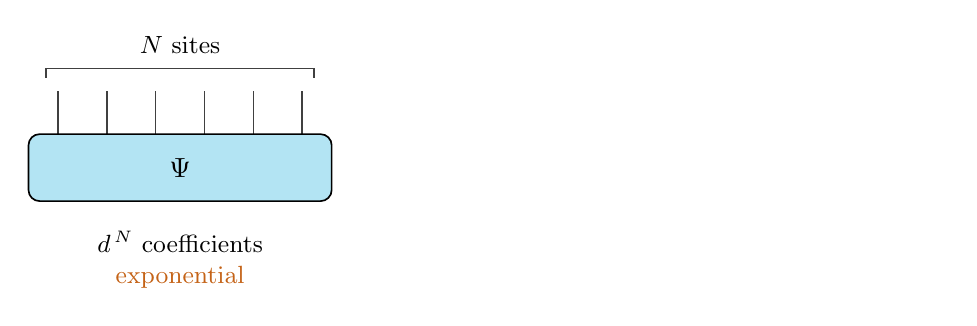
\begin{tikzpicture}[
    >={Stealth[round,length=2.2mm]},
    leg/.style={draw=black!75, line width=0.5pt},
    W/.style={circle, draw=black, fill=tnbulk, line width=0.5pt, minimum size=5.2mm, inner sep=0pt},
    tag/.style={font=\small},
  ]

  %% ---------------- generic state: one big tensor ----------------
  \begin{scope}
    \foreach \i in {0,...,5} { \draw[leg] ({\i*0.62},0) -- ({\i*0.62},0.55); }
    \node[draw=black, fill=tnbulk!45, rounded corners=4pt, line width=0.6pt,
          minimum width=3.85cm, minimum height=0.85cm]
          at ({2.5*0.62},-0.42) {$\Psi$};
    \draw[black!75, line width=0.6pt]
      (-0.15,0.72) -- (-0.15,0.84) -- (3.25,0.84) -- (3.25,0.72);
    \node[tag, anchor=south] at (1.55,0.90) {$N$ sites};
    \node[tag, anchor=north] at ({2.5*0.62},-1.10)
      {$d^{\,N}$ coefficients};
    \node[tag, tnbnd, anchor=north, font=\small] at ({2.5*0.62},-1.55)
      {exponential};
  \end{scope}

  %% ---------------- arrow ----------------
  \draw[->, opacity=0, text opacity=0, line width=1.1pt, black!70] (4.35,-0.42) -- (6.05,-0.42)
    node[midway, above=3pt, tag] {factorise};

  %% ---------------- MPS ----------------
  \begin{scope}[xshift=6.8cm, opacity=0, text opacity=0]
    \foreach \i in {0,...,5} {
      \draw[leg] ({\i*0.85},0) -- ({\i*0.85},0.55);
    }
    \draw[leg, line width=0.7pt] (0,0) -- ({5*0.85},0);
    \foreach \i in {0,...,5} { \node[W] at ({\i*0.85},0) {}; }
    % chi lives on the virtual bond BETWEEN two tensors;
    % d sits ON TOP of an open physical leg so the two are not confused
    \node[tag, anchor=south] at ({2.5*0.85},0.10) {$\chi$};
    \node[tag, anchor=south] at (0,0.60) {$d$};
    \node[tag, anchor=north] at ({2.5*0.85},-0.68)
      {$N \chi^2 d$ parameters};
    \node[tag, tnbulk!60!black, anchor=north, font=\small] at ({2.5*0.85},-1.13)
      {polynomial};
  \end{scope}

\end{tikzpicture}
\end{document}
